% LaTeX Template for Project Report, Version 2.0
% (Abstracted from a Major Project Report at CSED, NIT Calicut but can be
% modified easily to use for other reports also.)
%
% Released under Creative Commons Attribution license (CC-BY)
% Info: http://creativecommons.org/licenses/by/3.0/
%
% Created by: Kartik Singhal
% BTech CSE Batch of 2009-13
% NIT Calicut
% Contact Info: kartiksinghal@gmail.com
%
% It is advisable to learn the basics of LaTeX before using this template.
% A good resource to start with is http://en.wikibooks.org/wiki/LaTeX/
%
% All template fields are marked with a pair of angular brackets e.g. <title here>
% except for the ones defining citation names in ref.tex.
%
% Empty space after chapter/section/subsection titles can be used to insert text.
%
% Just compile this file using pdflatex after making all required changes.

\documentclass[12pt,a4paper,margin=0in]{report}

\usepackage{geometry}
\geometry{a4paper, portrait, margin=1in}
\usepackage{tabulary}
\usepackage{longtable}
\usepackage{varioref}
\usepackage[pdftex]{graphicx} %for embedding images
\usepackage{url} %for proper url entries
\usepackage[bookmarks, colorlinks=false, pdfborder={0 0 0}, pdftitle={A
Fencing Competition Results Web Service}, pdfauthor={Matthew Carus},
pdfsubject={BSc Computing and IT}, pdfkeywords={Open University,
Computing, IT, Report, TM470}]{hyperref}
%for creating links in the pdf version and other additional pdf attributes, no effect on the printed document
\usepackage[final]{pdfpages} %for embedding another pdf, remove if not required
\usepackage{listings} %for including source code
\usepackage{color} %for including source code

\usepackage[toc,page]{appendix}

\usepackage{titlesec}
 
\titleformat
{\chapter} % command
[display] % shape
{\bfseries\Large\itshape} % format
%{\normalfont\huge\bfseries}
{}
% {Part \ \thechapter} % label
{0ex} % sep
{
    \rule{\textwidth}{2pt}
    \vspace{1ex}
    \centering
    \thechapter\quad
} % before-code
[
\vspace{-0.5ex}%
\rule{\textwidth}{0.3pt}
] % after-code
\titlespacing*{\chapter}{0pt}{-50pt}{40pt}

\usepackage[round]{natbib}
\bibliographystyle{abbrvnat}
\setcitestyle{authoryear,open={(},close={)}}

\usepackage{csquotes}

\begin{document}
\renewcommand\bibname{References} %Renames "Bibliography" to "References" on ref page

%include other pages
\begin{titlepage}

\begin{center}

\textup{\small {\bf TM470 Project Report}}\\[0.2in]

% Title
\Large \textbf {A Fencing Competition Results \\ Web Service}\\[0.2in]

       \small \emph{Submitted in partial fulfillment of\\
        the requirements for the award of the degree of}
        \vspace{.2in}

       {\bf Bachelor of Science \\in\\ Computing and IT}\\[0.2in]

% Submitted by
\normalsize Submitted by \\
\begin{table}[h]
\centering
\begin{tabular}{lr}\hline 
\\
Matthew Anthony Carus & B3951972 \\ \\ \hline 
\end{tabular}
\end{table}

\vspace{.1in}
Under the guidance of\\
{\textbf{Prof. Peter Smith}}\\[0.2in]

\vfill


% Bottom of the page
% 
\includegraphics[width=0.36\textwidth]{Open_University_coat_of_arms}\\[0.1in]

%\begin{minipage}[t][][t]{0.45\textwidth}
\begin{center}
%
\includegraphics[width=3cm]{ou_cmyk_masterlogo_29mm.jpg}\\[0.4in]

\includegraphics[width=3cm]{Open_University_coat_of_arms.png}\\[0.4in]
\Large{Department of Computing and IT}\\
\normalsize
\textsc{The Open University}\\
Milton Keynes, United Kingdom \\
\vspace{0.2cm}
\end{center}
%\end{minipage}%
%\begin{minipage}[t][][t]{0.45\textwidth}
\begin{center}
\textsc{In collaboration with}\\[0.2in]

\includegraphics[width=3cm]{british-fencing.png}\\[0.1in]
\Large{British Fencing}\\
\normalsize
London, United Kingdom \\
\vspace{0.2cm}
\end{center}
%\end{minipage}%

\end{center}


\end{titlepage}

% \newpage
\thispagestyle{empty}

\begin{center}

\huge{Department of Computing and IT}\\[0.5cm]
\normalsize
\textsc{The Open University}\\[2.0cm]

\emph{\LARGE Certificate}\\[2.5cm]
\end{center}
\normalsize This is to certify that this is a bonafide record of the project
presented by the student whose name is given below during 2016 in partial fulfilment of the requirements of the degree of Bachelor of Science in Computing
and IT.
[1.0cm]
\begin{table}[h]
\centering
\begin{tabular}{lr}
Student Name & PI Number \\ \\ \hline

Matthew Anthony Carus & B3951972
\end{tabular}
\end{table}

\vfill


% Bottom of the page
\begin{flushright}
<Tutor name here>\\
(Tutor)\\[1.5cm]
Leonor Barroca \\
(Module Team Chair)
[1.5cm]
\today
\end{flushright}
\vspace{2in}
\begin{abstract}

<Abstract here>

\end{abstract} 


\pagenumbering{roman} %numbering before main content starts
\tableofcontents
\listoffigures
\listoftables

\newpage
\pagenumbering{arabic} %reset numbering to normal for the main content

\chapter{Problem Definition}

<Problem Definition here>
 %objective changed to problem definition
% \chapter{Introduction}

\section{Background and Recent Research}
\subsection{<any sub section here>}

\subsection{Literature Survey}

\subsubsection{<Sub-subsection title>}
some text \citep{knuthwebsite} \citet{latexcompanion}, some more text

\subsubsection{<Sub-subsection title>}
even more text\footnote{<footnote here>}, and even more.

\section{Motivation}
 %literature survey included in this
\chapter{Project Goals} \label{goals}

The goal of this project is to produce a working system that meets 
requirements that will later be identified. The system will be designed and
built using the knowledge that I have built up during the course of my Open
University studies. As such it is likely to be designed using UML and
implemented using Java. The specific elements that I will deliver will be as
follows:
\begin{itemize}
  \item Output from the modelling phase of the project. This will include
  a domain model, class models etc.
  \item A database schema, designed to best practices, that will be used to
  store all of the relevant information derived from the modelling exercise.
  \item A working database implementing the database schema, populated with real
  data.
  \item An API to the database such that data can be added to the database and
  data already in the database can be retrieved. The API should use standard
  data formats for accepting data and for presenting it. This API should be
  designed in such a way that it can be extended in the future to allow for
  other operations (for example updating data already in the database, searching for data etc.)
  \item A web interface to allow viewing of the data held within the database.
\end{itemize}
Some activities will specifically be excluded from the scope of the project.
This is primarily due to time constraints but also to properly complete the
activities would require more knowledge than I have gained during the course of
my studies. If during the course of my research and development work it becomes
evident that this can be added in a trivial manner then they may later be
re-introduced into the scope of the project. These are:
\begin{itemize}
  \item API Security. It is anticipated that I will not implement access control
  on the API. A live deployment of the API will either require that
  authentication be added or an application firewall be utilised to only permit
  certain operations.
  \item Web interface to advanced operations. It is accepted that the web
  interface will only allow viewing of the data exposed by the API. In order to
  add data to the database the API will be used directly, rather than via a web
  interface.
\end{itemize}
Aside from the domain research needed for the modelling phase and associated
requirements generation, the following additional research tasks have been
identified:
\begin{enumerate}
  \item Research into the data formats that will be used to populate the
  database via the API, and the desired output formats from the API.
\end{enumerate}
The output of this research is presented in section \ref{research} beginning on
page
\pageref{research}

\chapter{Project Plan}

% \section{Gantt Chart}
% \def\svgwidth{350px}
%\input{gantt.pdf_tex}
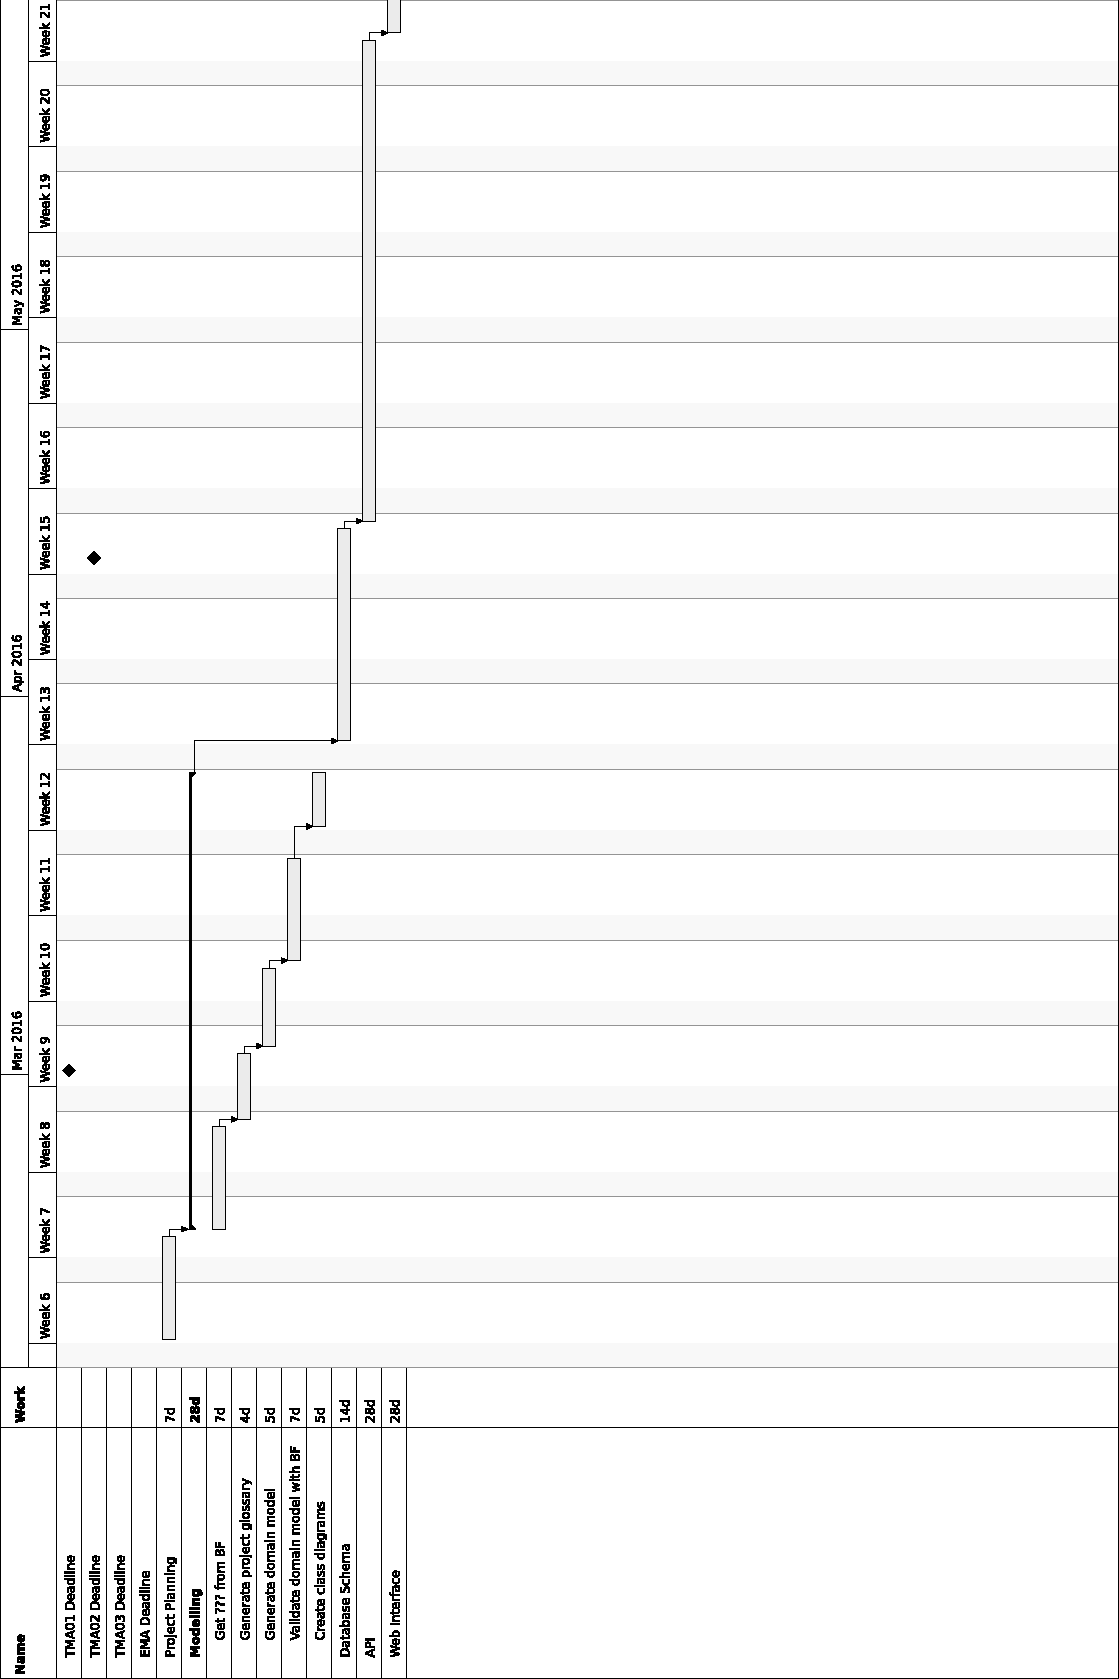
\includepdf{gantt-p1.pdf}
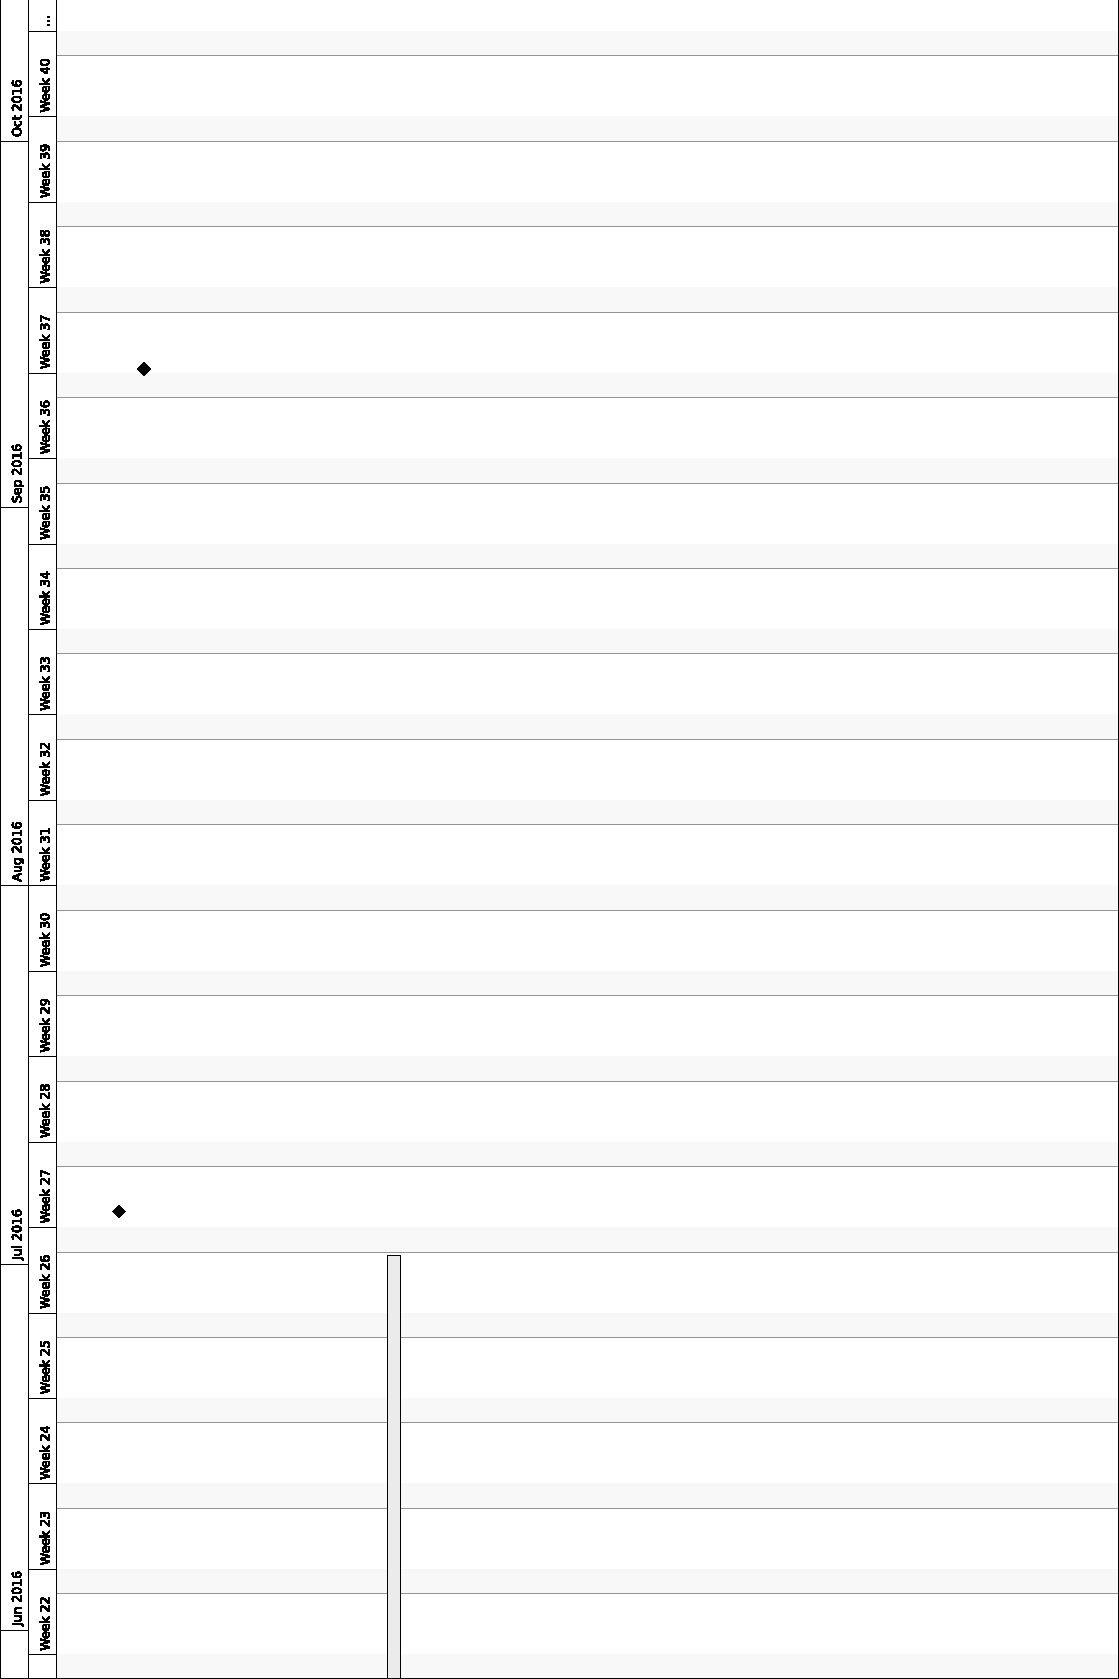
\includepdf{gantt-p2.pdf}
\chapter{Research} \label{research}

\section{Data Formats}
From speaking to Katie Rhodes (British Fencing) and to other competition
organisers, it has become clear that one of two pieces of software are used to
organise fencing competitions. These are called \textit{Engarde} and
\textit{Fencing Time}. Both programs have the ability to output XML files
detailing the results of the competition \citep{engardewebsite} and
\citep{fencingtimewebsite}. XML samples from each program are supplied in
Appendix \ref{appendix-sample-fencing-xml} on page
\pageref{appendix-sample-fencing-xml}. Clearly, the two programs use different
formats.

For the output format from the API, it would be possible to re-use one
(or both) of these two formats, or a different format could be used. If a
different format is chosen then it could either be a format that I create
specifically for this system, or it could be a format published elsewhere.
Further internet-based research has indicated that there are standards in
existence for representing sports data. One such standard is known as SportsML,
the current version of which (as of Feb 2016) is SportsML-G2. This standard is
defined by the \textit{International Press Telecommunications Council (IPTC)}. I
contacted the IPTC via their developer forums to ask if fencing data could be
represented in SportsML format and the response was that it should be able to be
represented but no-one was aware of anyone currently using SportsML for fencing
data. Two interesting responses were received from the initial posting, one from
Steve Potts at the \textit{BBC} and another from Jean F\`{e}vre of
\textit{L'Agence France-Presse (AFP)}.\\
Steve Potts, in an email to me stated that the BBC did use SportsML as their
favoured format for receiving data, he also stated:
\begin{displayquote}
The BBC are interested in the concept of local generated
sports stats (compare with user generated, which it is not), and also in publishing stats for
lesser-participated sports. The effort we expend in obtaining and publishing
stats is naturally weighted towards the more popular sports, so we are
investigating opening channels (with a lower barrier to entry) of sports stats
ingest from outside our primary suppliers. Fencing isn't included in our
supplier contracts, so creating a vocabulary for it removes one barrier for us
to publish its stats. Our ideal scenario is for us to ingest a routine automated
SportsML feed from British Fencing for fixtures, results and standings to appear
across the BBC Website, Mobile App, Red Button TV, Connected TV.
\citep{pottsemail20160202}
\end{displayquote}
From this I take that the BBC would be interested in integrating with the system
I am to build in order to receive data automatically from British Fencing. This
is something the British Fencing are quite excited about! Conversely, Jean
F\`{e}vre, again in an email, states:
\begin{displayquote}
I am in SportML group since long time but I don’t like SportML too much because
it’s very complex and it must be adapted to each sport.
I work with IOC on Olympic Games since very long time (1988) and we (IOC, ASOIF,
many international federations…) have defined ODF XML format.
For Rio games we will receive ODF 2. \citep{ferveemail20160203}
\end{displayquote}
After studying at the two formats, I would dispute F\`{e}vre's assertion that
SportsML is very complex - I understood it more quickly than the ODF format.
It is clear that there are two competing formats and it makes sense for me to
decide to support primarily one format, with support for the second being made
possible if it is able to be added.
One outstanding issue I had to face before making a decision on my primary data
format was that of whether or not SportsML would actually support fencing data
or not. As suggested by members of the SportML development group, I decided to
jump in at the deep end and actually produce a valid SportsML file with fencing
data in it. This file is available in Appendix
\ref{appendix-sample-fencing-sportsml} on page
\pageref{appendix-sample-fencing-sportsml} I made a copy of this file available
to the SportsML group for their comments, which were supportive. There remained
a small issue of embedding the weapon used for a particular competition in the
format (something that is not taken care of in the core SportsML standard) but
I'm confident that a solution can be found for that as the standard is easily
extensible.

\chapter{Models}
\section{Grammatical Parse} \label{section:gramaticalParse}
After consultation with British Fencing, I was directed to a useful resource
which describes how fencing competitions operate \citep{bfcompguide}. Not
all of this document is relevant but the sections that are are reproduced
below, with \textbf{nouns} in bold and \underline{verbs} underlined. Only the
nouns and verbs deemed to be directly relevant to the process of competing in a
competition have been included.
\begin{displayquote}
Check In: All \textbf{competitions} start by \textbf{fencers}
visiting the \textbf{check in desk} \underline{to confirm} that they
are present. Don’t miss this bit out - your \textbf{entry}
will \underline{be scratched}.
When \underline{checking in}, \textbf{fencers} are required to show
their \textbf{British Fencing card}. See the box (right) for
details. This carries \textbf{insurance}. Without it, you
may not fence. Fencing usually starts about 30 - 60 minutes
after \underline{check in} closes.
Pools: After \textbf{check in}, \textbf{competitors} are divided
into “\textbf{pools}” - groups of 5 - 7 \textbf{fencers} who all
\underline{fence} each other up to 5 \textbf{hits}. (4 \textbf{hits} for some
under 9 \textbf{competitions}). Time is limited to 2 or 3
minutes. Sometimes there may be two rounds of
\textbf{pools}, particularly in \textbf{age group competitions}.
Direct Elimination: The \textbf{results} of the \textbf{pools}
are used to \underline{seed} the \textbf{knockout phase} of the
\textbf{competition}. In some \textbf{competitions}, up to 30\%
of the \textbf{fencers} who did worst are \underline{eliminated}, but
in most cases all \textbf{fencers} \underline{go through} to the \textbf{direct
elimination (DE)} stage.
The \textbf{DE} rewards \textbf{fencers} who do well in the
\textbf{pool} stages, and keeps the strong \textbf{fencers} apart
until near the end of the \textbf{competition}. In a
\textbf{competition} with 64 \textbf{entrants}, the first round of
DEs would see 1st place fence 64th, 2nd place
fence 63rd and so on. If the number of
\textbf{entrants} is not a power of 2, (ie 8, 16, 32, 64
etc) then those \textbf{fencers} who did best in the \textbf{pools}
will \underline{get a “\textbf{bye}”} through the first \textbf{DE} round. After
several \textbf{DE} rounds, there will only be two \textbf{fencers}
left - the \textbf{finalists}.
\textbf{Direct elimination} fights are up to 15 \textbf{hits} (adults)
10 \textbf{hits} (under 13s) or 8 \textbf{hits} (under 9s). \textbf{DE fights}
are normally 3 x 3 minutes (sometimes less for \textbf{younger
fencers}) with a 60 second break between \textbf{periods}.
\end{displayquote}
\section{Project Glossary} \label{section:projectGlossary}
From the grammatical parse in section \vref{section:gramaticalParse} a project
glossary can be compiled. As a part of this, I removed all duplicate words,
plurals and synonyms, choosing the most appropriate word from any sets of synonyms as the noun or verb to represent
that entity/action. Note that synonyms in this sense are not necessarily true
synonyms but are equivalent terms in the context of fencing and fencing
competitions. Objects that have been identified as being a synonym of another
object, but not a complete synonym have had \textit{(sub-type)} appended to them
in the synonym list. The description of the words comes either from the text
above, from basic internet searching, or from my own knowledge of the sport.
\begin{center}
\begin{longtable}[l]{| p{.20\textwidth} | p{.80\textwidth} |} 
 \caption{\label{tab:ProjectGlossary}Project Glossary}
\hline
\textbf{Nouns} & \\ 
 Competition & An over-arching event at which one or more events
 take place \\
 & \textit{synonyms: age group competition (sub-type)} \\ 
 Fencer & An individual (human being) who competes in a fencing
 competition \\
 & \textit{synonyms: competitor, entrant, finalists (sub-type),
 younger fencers (sub-type)} \\
 Check-in desk & The location that fencers present themselves to
 in order to confirm that they will take part in a competition \\
 Entry & The link between a fencer and a competition \\
 British Fencing Card & A form of identity card indicating that a
 fencer has membership of British Fencing, and by extension is insured to
 compete \\
 & \textit{synonyms: insurance} \\
 Hit & The act of one fencer striking another and scoring a point \\
 Result & A listing of fencers in order of their measured performance in a 
 particular round \\
 Direct Elimination & The phase of a competition where defeating
 another fencer results in their elimination from the competition and your
 promotion to the next round. \\
 & \textit{synonyms: DE, knockout phase} \\
 Bye & The act of progressing through a round of the Direct
 Elimination stage of the competition without having to face another fencer.
 This is used in the event that the number of fencers is not a power of 2. \\
 Bout & An individual fencing match between two fencers \\
 & \textit{synonyms: fight} \\
 Period & A time-based subdivision of a bout \\
 Poule & A small grouping of fencers who all fence against one
 another in a series of bouts. \\
 & \textit{synonyms: pool} \\ 
 Event & A tournament in which fencers of the same gender, age
 group and weapon fence \\
 \textbf{Verbs} & \\
 Check In & The act of a fencer confirming that they have arrived at the venue
 of the competition and they intend to compete in it. \\
 & \textit{synonyms: to confirm (attendance at the competition)} \\
 Be Scratched & To be removed from the competition without competing \\
 Fence & The act of one fencer engaging in a fencing bout with another fencer \\
 & \textit{synonyms: fight} \\
 Seed & To use the results of one or more round(s) of competition to determine
 the structure of the next round. \\
 Eliminated & To be removed from the competition as a result of loosing a bout
 in a Direct Elimination round, or (in some cases) not being ranked high enough
 after a round of Poules \\
 Go Through & To progress from one round to the next, either by being ranked
 high enough after a poules round, or by winning a Direct Elimination bout \\
 Get a Bye & Be in receipt of free passage from one round of Direct
 Elimination to the next, without having to face another fencer. This is used in
 the case that the number of competitors in a round of Direct Elimination is not
 a power of 2 \\
 \hline
\end{longtable}
\end{center}
\section{Business Processes} \label{section:businessProcesses}
I have decided that for the purposes of this project, modelling the business
processes associated with the process of a fencer taking part in a competition
is not appropriate. The reason for this is that the software system will not
seek to implement these processes, but rather be an archive or the results of
these processes. Other software (such as Engarde and Fencing Time, mentioned in
section \vref{chapter:research}) already implement these processes. The
business processes that I will model will be the process by which data gets
added to the system and viewed by users of the system.
\section{Use Case Diagram} \label{section:useCaseDiagram}
\begin{figure}[!ht]
  \centering
  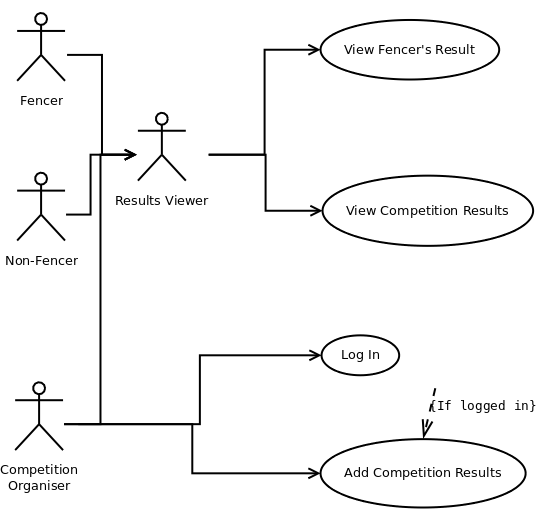
\includegraphics[width=10cm]{use_case_diagram.png}
  \caption{Use Case Diagram}
\end{figure}
\section{Class Diagram} \label{section:classDiagram}
As mentioned above, the project glossary includes terms relating to the actual
competition process. Some of these terms are relevant to a results hosting
service and some are not. Terms like \textit{Check-in desk} and
\textit{British Fencing Card } are only relavent during the actual competition
itself, therefore I have excluded them from the class diagram in
\vref{fig:classDiagram}.
\begin{figure}[!ht]
  \centering
  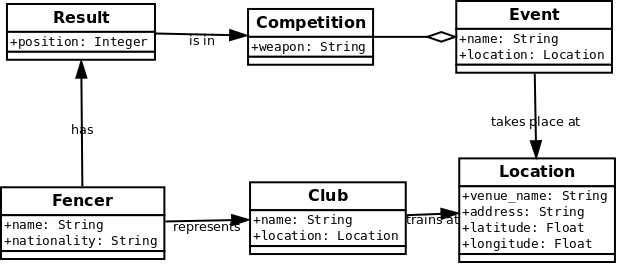
\includegraphics[width=10cm]{class_diagram.png}
  \caption{Class Diagram}
  \label{fig:classDiagram}
\end{figure}
\begin{figure}[!ht]
  \centering
  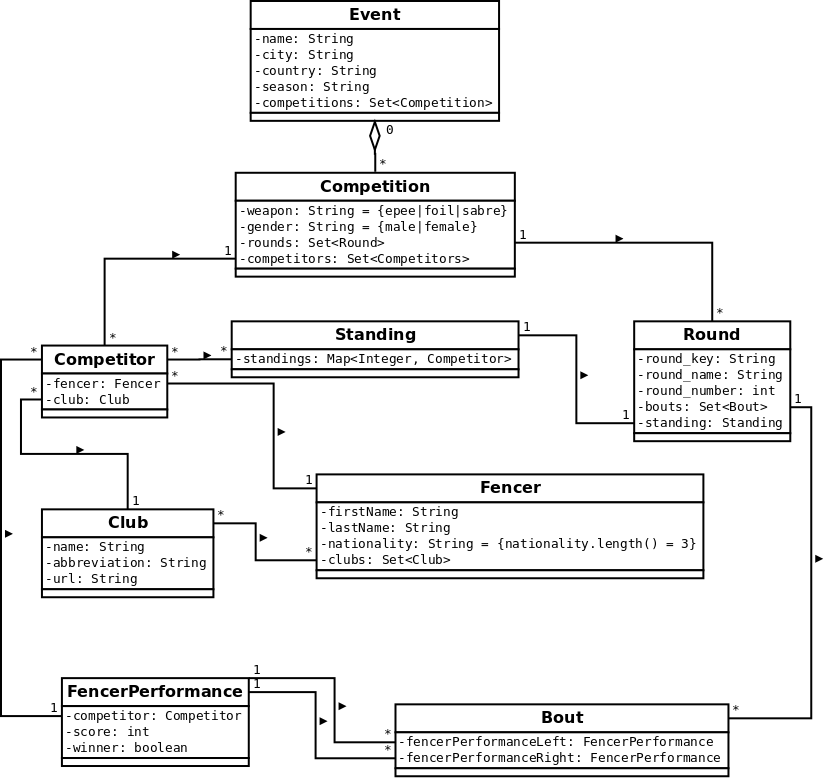
\includegraphics[width=12cm]{class_diagram_full.png}
  \caption{Full Class Diagram}
  \label{fig:classDiagramFull}
\end{figure}
\begin{figure}[!ht]
  \centering
  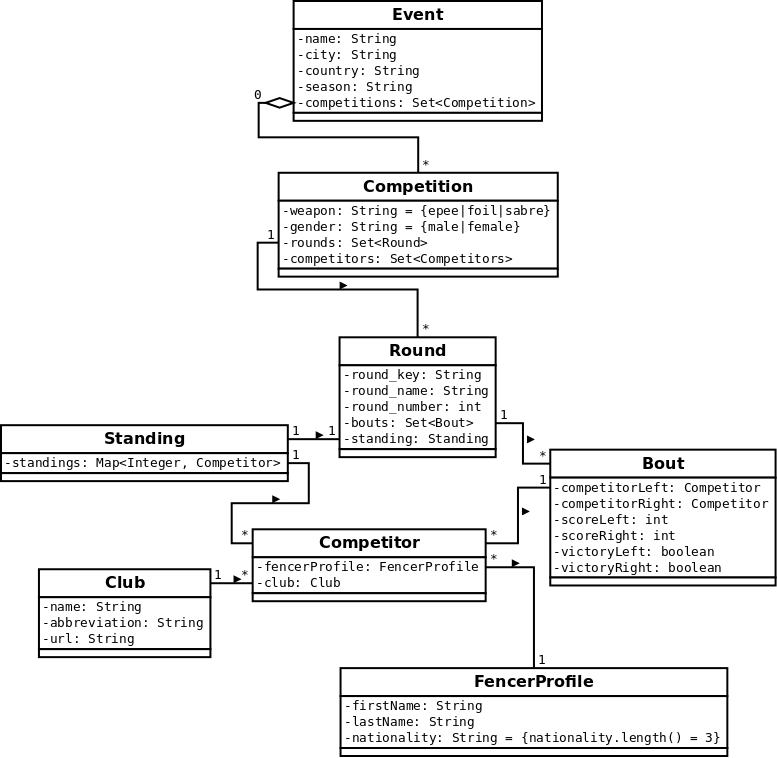
\includegraphics[width=10cm]{class_diagram_reduced.png}
  \caption{Reduced Class Diagram}
  \label{fig:classDiagramFull}
\end{figure}
The class diagrams in \vref{fig:classDiagramGeneratedNetFencingarchive}\footnote{Also available at
  http://github.com/mattcarus/something/here.png} and
\vref{fig:classDiagramGeneratedSportsml}\footnote{Also available at
  http://github.com/mattcarus/something/here.png} reflects what was actually coded in the
\(net.fencingarchive\) and \(sportsml\) packages and were generated
automatically (but re-arranged manually).
\begin{figure}[!ht]
  \centering
  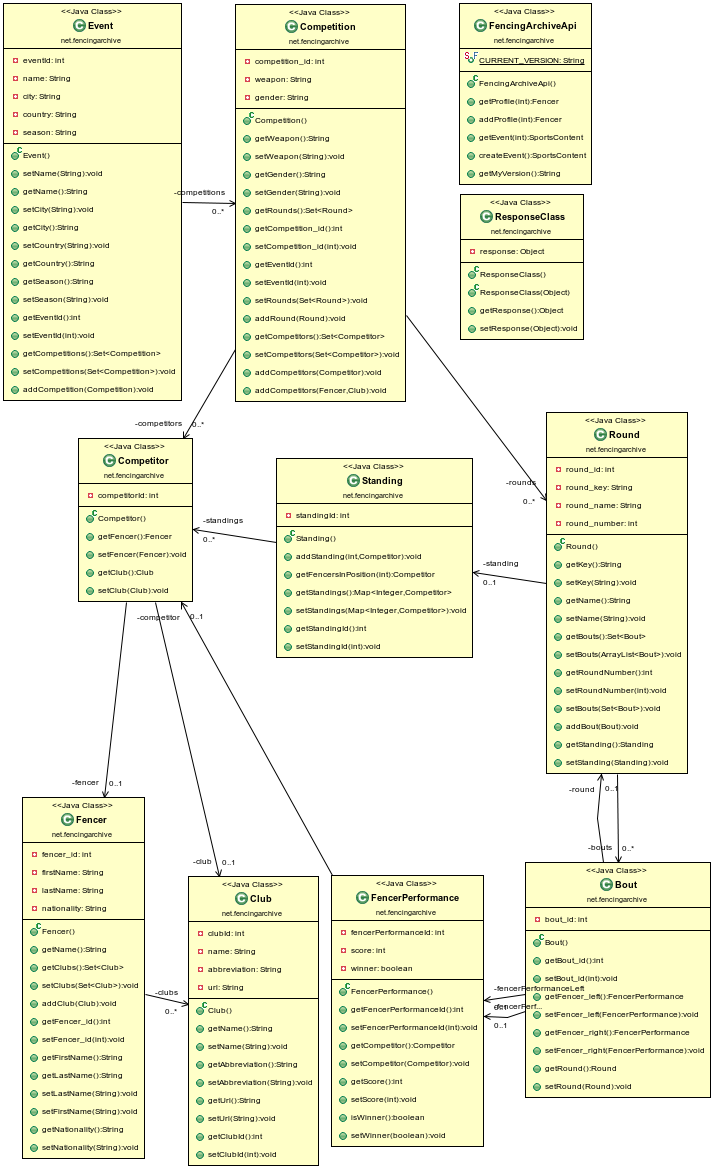
\includegraphics[width=\textwidth,height=0.9\textheight,keepaspectratio]{ObjectAid/class-diagram.png}
  \caption{net.fencingarchive Class Diagram - Generated from source code}
  \label{fig:classDiagramGeneratedNetFencingarchive}
\end{figure}
\begin{figure}[!ht]
  \centering
  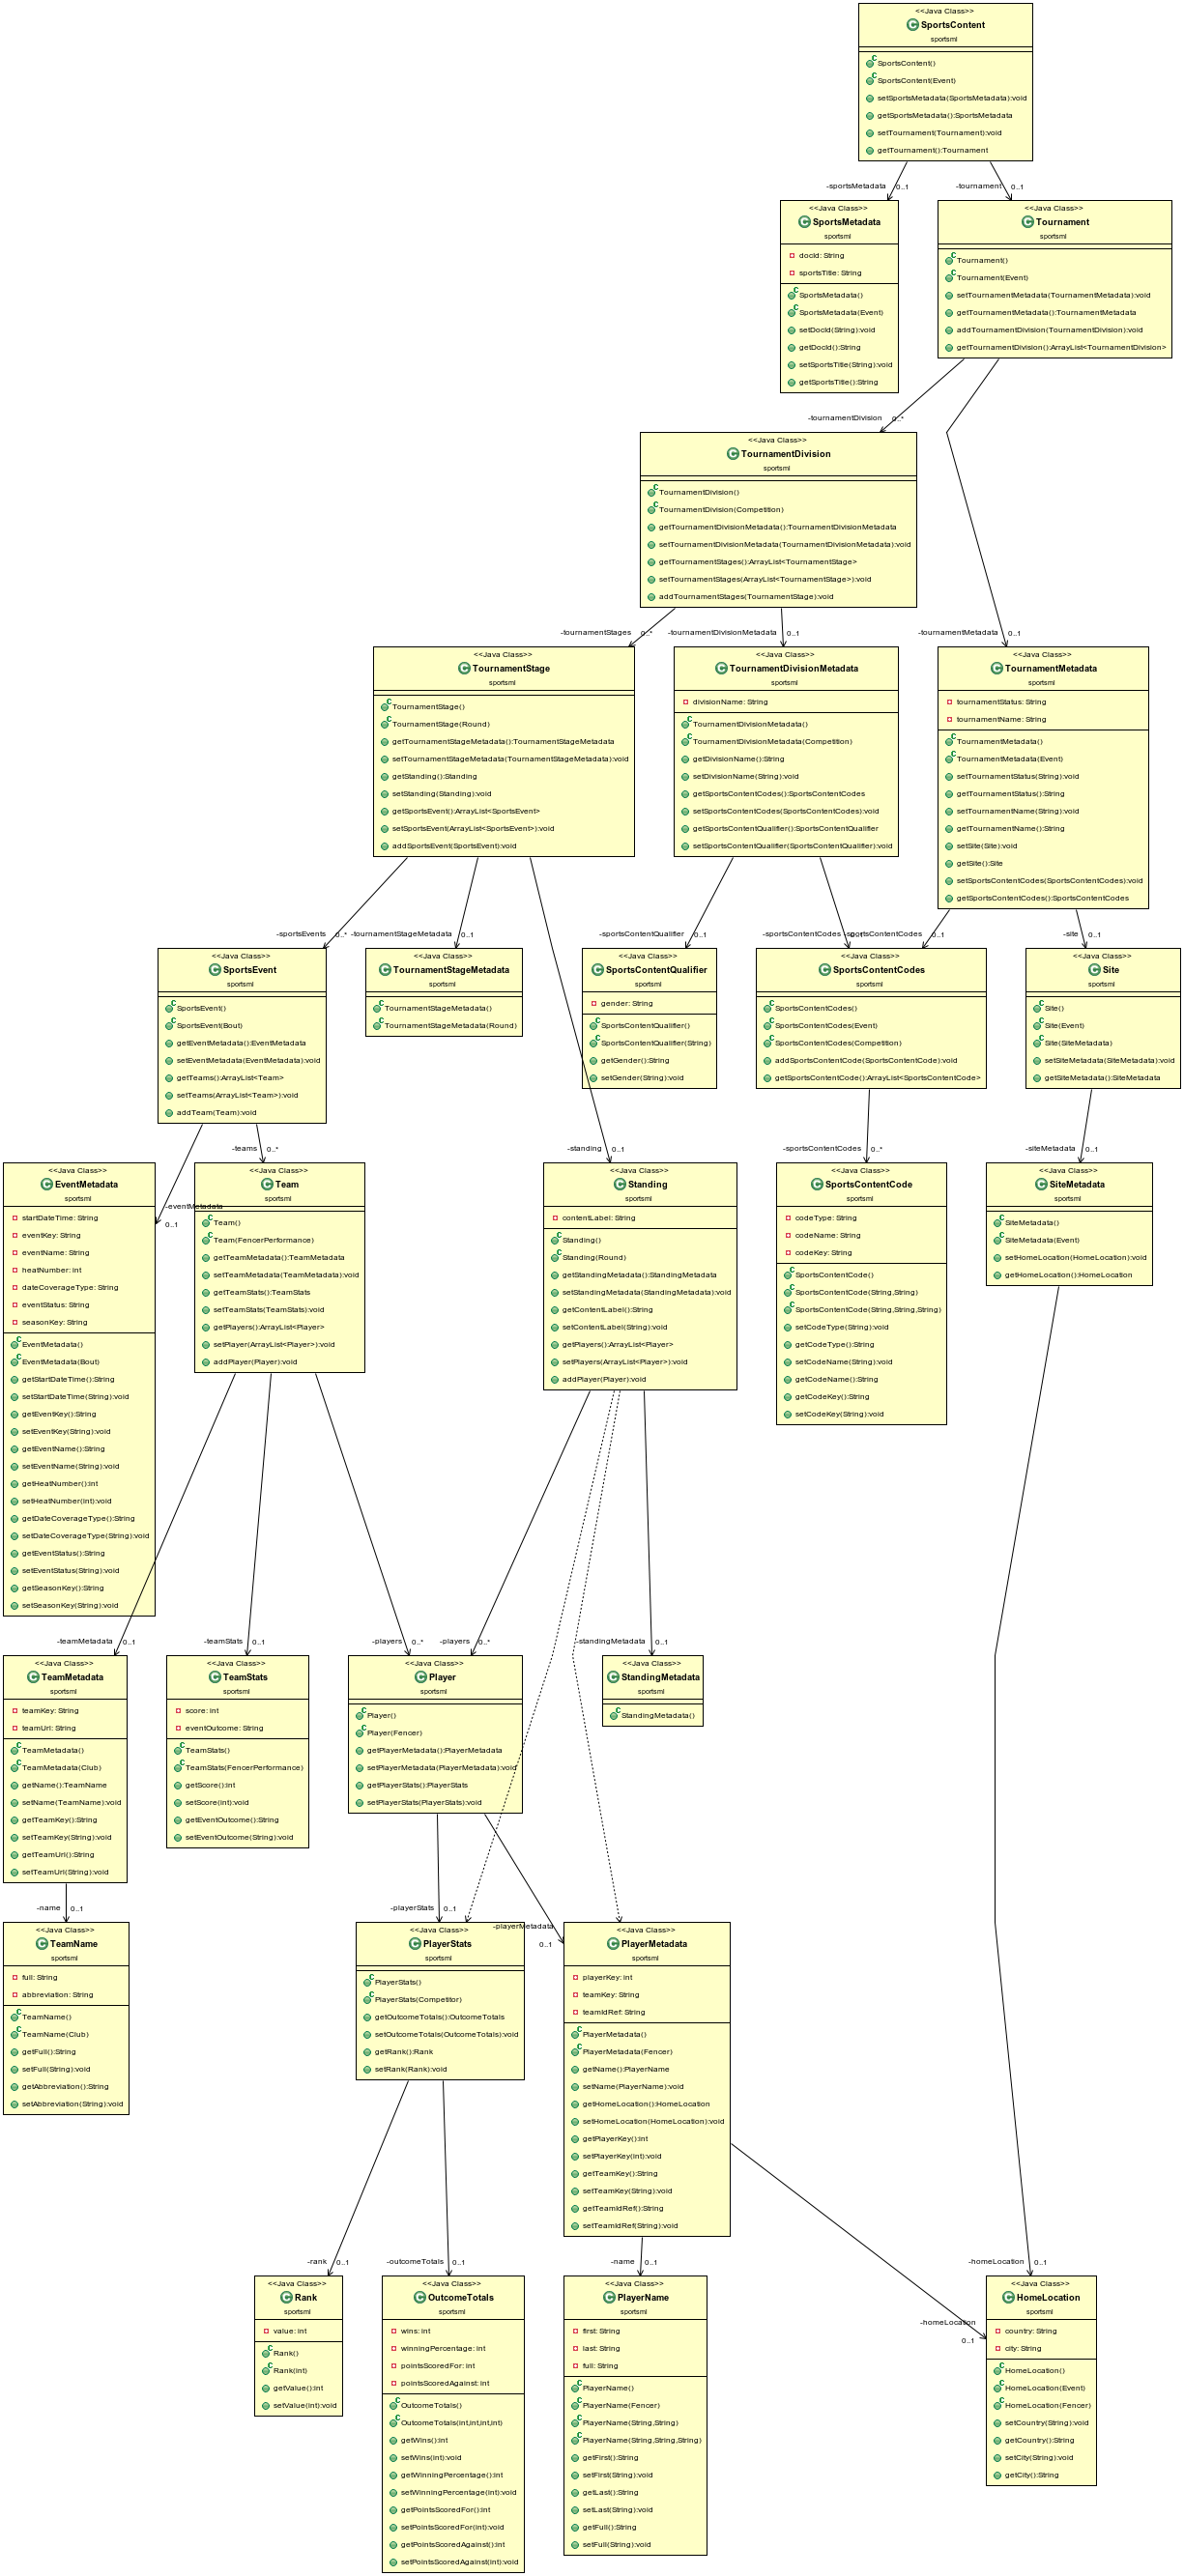
\includegraphics[width=\textwidth,height=0.9\textheight,keepaspectratio]{ObjectAid/class-diagram-sportsml.png}
  \caption{sportsml Class Diagram - Generated from source code}
  \label{fig:classDiagramGeneratedSportsml}
\end{figure}
\section{Database Design} \label{sectiondatabaseDesign}
\begin{figure}[!ht]
  \centering
  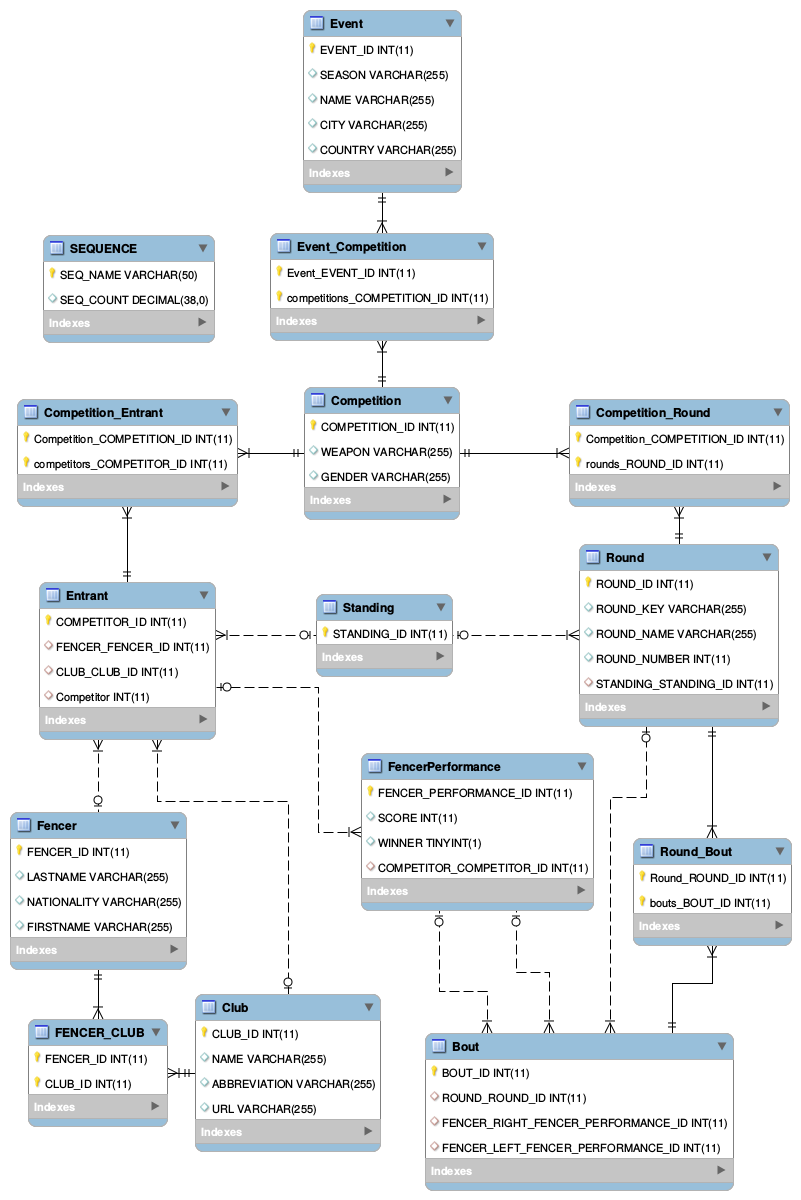
\includegraphics[width=15cm]{db-model.png}
  \caption{Database ER Model - as generated by MySQL Workbench}
  \label{fig:databaseERDesignGenerated}
\end{figure}

\chapter{Work Done}

\section{<Section title>}

\subsection{<Sub-section title>}

\subsection{<Sub-section title>}
some text\citep{einstein}, some more text
\subsection{<Sub-section title>}

\subsection{<Sub-section title>}

Refer figure \ref{fig:label}.

\begin{figure}[htb]
\centering

\includegraphics[scale=0.3]{glider} % e.g. insert ./image for image.png in the working directory, adjust scale as necessary
\caption{<Caption here>}
\label{fig:label} % insert suitable label, this is used to refer to a fig from within the text as shown above
\end{figure}

\subsection{<Sub-section title>}


\section{<Section title>}


\section{Source Code}

\definecolor{mygreen}{rgb}{0,0.6,0}
\definecolor{mygray}{rgb}{0.5,0.5,0.5}
\definecolor{annotationgray}{rgb}{0.25,0.25,0.25}
\definecolor{mymauve}{rgb}{0.58,0,0.82}

\lstset{ %
  backgroundcolor=\color{white},   % choose the background color; you must add \usepackage{color} or \usepackage{xcolor}
  basicstyle=\footnotesize,        % the size of the fonts that are used for the code
  breakatwhitespace=false,         % sets if automatic breaks should only happen at whitespace
  breaklines=true,                 % sets automatic line breaking
  captionpos=b,                    % sets the caption-position to bottom
  commentstyle=\color{mygreen},    % comment style
  deletekeywords={...},            % if you want to delete keywords from the given language
  escapeinside={\%*}{*)},          % if you want to add LaTeX within your code
  extendedchars=true,              % lets you use non-ASCII characters; for 8-bits encodings only, does not work with UTF-8
  frame=single,	                   % adds a frame around the code
  keepspaces=true,                 % keeps spaces in text, useful for keeping indentation of code (possibly needs columns=flexible)
  keywordstyle=\color{blue},       % keyword style
  language=Java,                 % the language of the code
  morecomment=[s][\color{annotationgray}]{@}{\ },	% for setting @Annotations to
  % grey
  numbers=left,                    % where to put the line-numbers; possible
  % values are (none, left, right)
  numbersep=5pt,                   % how far the line-numbers are from the code
  numberstyle=\tiny\color{mygray}, % the style that is used for the line-numbers
  rulecolor=\color{black},         % if not set, the frame-color may be changed on line-breaks within not-black text (e.g. comments (green here))
  showspaces=false,                % show spaces everywhere adding particular underscores; it overrides 'showstringspaces'
  showstringspaces=false,          % underline spaces within strings only
  showtabs=false,                  % show tabs within strings adding particular underscores
  stepnumber=1,                    % the step between two line-numbers. If it's 1, each line will be numbered
  stringstyle=\color{mymauve},     % string literal style
  tabsize=2,	                   % sets default tabsize to 2 spaces
  title=\lstname                   % show the filename of files included with \lstinputlisting; also try caption instead of title
}

\lstinputlisting{dummy_source.java}

% Trying an XML file
\lstinputlisting[language=XML]{../SportsML-G2/testing/example-2-open.xml}


\cleardoublepage
%\pagebreak
\phantomsection
\addcontentsline{toc}{chapter}{Acknowledgements}
\chapter*{Acknowledgments}
\vspace{1.0in}
<Acknowledgements here>


 

<Name here>

<Month and Year here>
{National Institute of Technology Calicut}
\newpage

\cleardoublepage
%\pagebreak
\phantomsection
\addcontentsline{toc}{chapter}{References}

%\bibliographystyle{agsm}
%\bibliography{references}

%\begin{thebibliography}{99}
%
%\bibitem{citation-1-name-here}<Name of the reference here>,\ \url{<url here>}
%
%\bibitem{citation-2-name-here}<Name of the reference here>,\ \url{<url here>}
%
%\end{thebibliography}


\bibliography{references}

\begin{appendices}
\chapter{Sample Fencing XML} \label{appendix-sample-fencing-xml}

This is just a placeholder file, need to include Engarde XML and FencingTime XML
files here

\section{Engarde XML} \label{engarde-xml-sample}
\lstinputlisting[language=XML]{../SportsML-G2/testing/example-2-open.xml}
\section{FencingTime XML} \label{fencingtime-xml-sample}
\lstinputlisting[language=XML]{../SportsML-G2/testing/example-2-open.xml}

\chapter{Sample SportsML} \label{appendix-sample-fencing-sportsml}
\section{Original Sample SportsML file of Fencing Data} \label{sportsml-sample}
\lstinputlisting[language=XML]{../SportsML-G2/testing/example-2-open.xml}
\section{Sample SportsML file after Advice from SportsML Developers}
\label{sportsml-sample-2}
\lstinputlisting[language=XML]{../SportsML-G2/testing/example-2-open-2.xml}
\end{appendices}

\end{document}
